\documentclass[a4paper, 12pt]{article}

% Paquetes básicos para idioma y codificación
\usepackage[utf8]{inputenc}
\usepackage[T1]{fontenc}
\usepackage[spanish]{babel}

% Paquete para insertar imágenes
\usepackage{graphicx}

% --- PAQUETE NUEVO PARA FORZAR LA POSICIÓN DE LAS IMÁGENES ---
\usepackage{float} 

% Paquete para que el índice tenga enlaces clickeables
\usepackage[colorlinks=true, linkcolor=black, urlcolor=blue]{hyperref}

% Configuración del título
\title{Memoria de Prácticas: Ingeniería de Servidores}
\author{Juan Reche Aguilar}
\date{\today}

\begin{document}

% Genera la portada con el título
\maketitle
\clearpage % Usamos clearpage en lugar de newpage

\section{Ejercicio 2: Configuración de red}

% Imagen 1 (Fíjate en la H mayúscula)
\begin{figure}[H]
    \centering
    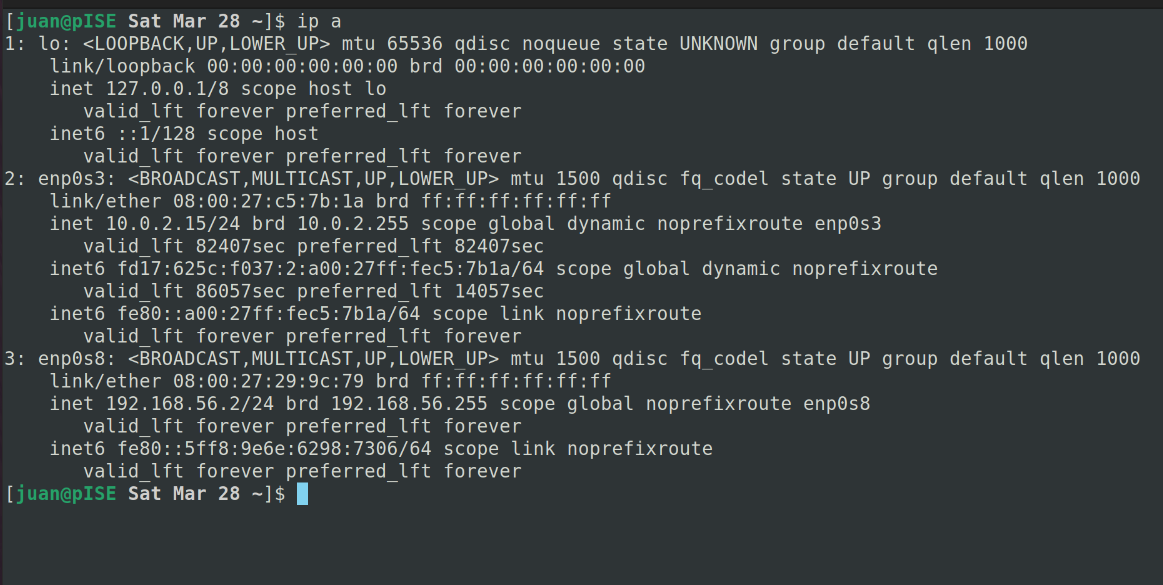
\includegraphics[width=0.8\textwidth]{../ej2/ej2_1.png}
    \caption{configuración red del servidor con ip a}
\end{figure}

% Imagen 2
\begin{figure}[H]
    \centering
    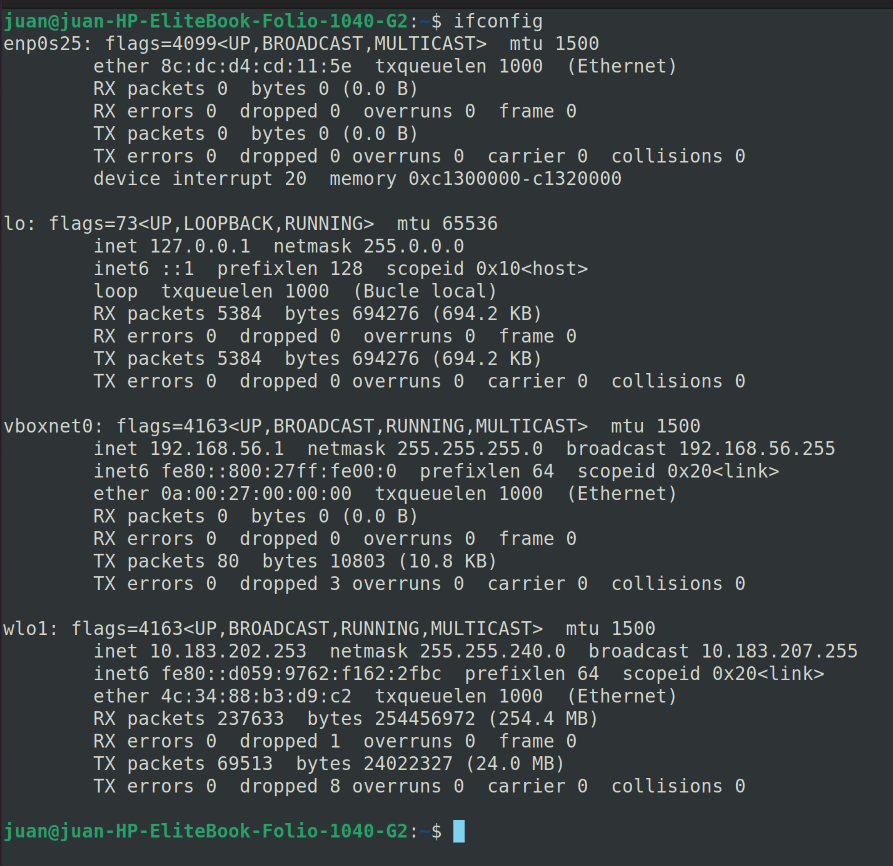
\includegraphics[width=0.8\textwidth]{../ej2/ej2_2.png}
    \caption{configuración red del host con ifconfig}
\end{figure}

% Imagen 3
\begin{figure}[H]
    \centering
    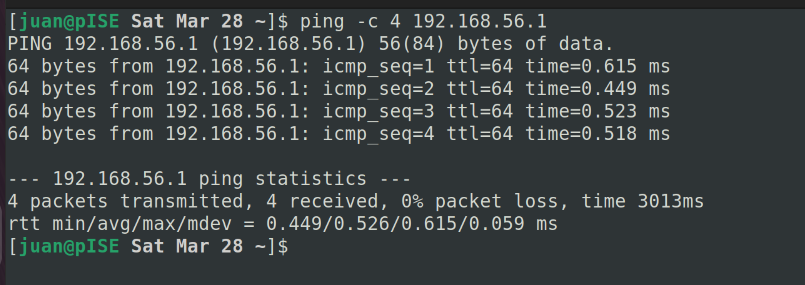
\includegraphics[width=0.8\textwidth]{../ej2/ej2_3.png}
    \caption{Desde la VM hacemos ping al ordenador fisico}
\end{figure}

% Imagen 4
\begin{figure}[H]
    \centering
    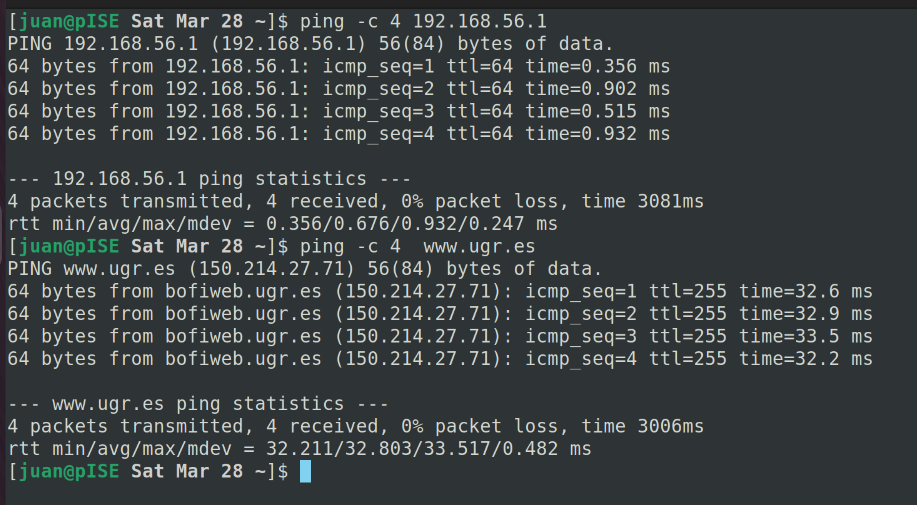
\includegraphics[width=0.8\textwidth]{../ej2/ej2_4.png}
    \caption{Desde la VM hacemos ping a la ugr}
\end{figure}

% Imagen 5
\begin{figure}[H]
    \centering
    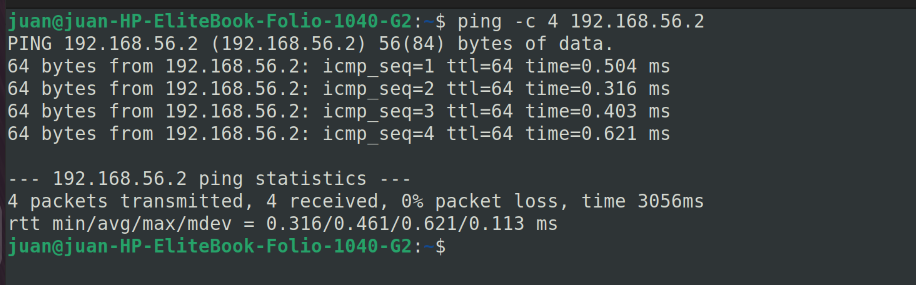
\includegraphics[width=0.8\textwidth]{../ej2/ej2_5.png}
    \caption{Desde el ordenador fisico hacemos ping a la VM}
\end{figure}

\end{document}
